\section{Introduction}\label{sec:introduction}

Preventable Medical Errors (\PMEs{}) characterized by
incorrect intended treatment, or incorrect executions of intended
treatment present a significant challenge in Healthcare
\cite{RodziewiczStatsPearls18}. According to a seminal report on the subject
\cite{DonaldsonBook00}, in 1997,
between 44,000 and 98,000 deaths were estimated to have been caused by \PMEs{} in
the United States alone. A more recent study analyzed data from the eight-year
period between 2000 and 2008, and estimated that in 2013, the number of deaths
caused by \PMEs{} was more than 250,000, making \PMEs{} the third-leading
cause of death in the United States \cite{MakaryBMJ16}.
The adverse effects of \PMEs{} extend beyond patient outcomes.
One study estimated the financial burden of \PMEs{} to the United States to be
19.5 billion dollars in 2008 \cite{AndelJHCF12}. According to the authors of
\cite{RodziewiczStatsPearls18}, \PMEs{} caused psychological effects such
as anger and guilt in healthcare providers (\HCPs{}), adversely impacting their mental
health.

One strategy to mitigate \PMEs{} is to utilize evidence-based statements
published by hospital and medical associations that codify recommended
interventions for various clinical scenarios called Best Practice Guidelines (\BPGs{})
\cite{field1990clinical}. High quality guidelines are routinely updated to account for
 results from clinical trials and advances in medicine, and make the latest
 diagnosis and treatment information accessible to providers \cite{SteinbergNAP11}.

While \BPGs{} have the potential to reduce medical errors, their effectiveness hinges
on the adherence of healthcare providers to them.
For example, consider Advanced Cardiac Life Support (\ACLS{}): a \BPG{} published
by the American Heart Association (AHA) for management
of a life threatening condition called in-hospital cardiac arrest (IHCA) \cite{AHAGuidelineAdult, AHAGuidelinePed}. Studies suggest that management
of IHCA in 30\% of adult, and 17\% of pediatric cases deviates from the
AHA-prescribed \BPG, resulting in worse patient outcomes \cite{Ornato2012DeviationAdult,Wolfe2020DeviationPediatric,
Crowley2020DeviationAdult,Honarmand2018Adherence,Mcevoy2014Adherence}.

While \BPG{}-adherence is difficult to achieve in
practice \cite{RandJAMA99,DavisCMAJ97},
integrating \BPGs{} with existing patient care-flow,
and making them readily-accessible when required can improve adherence \cite{WoolfBMJ99}.
To this end, hospitals commission computerized Decision Support Systems (\CDSSs{})
that codify \BPGs{} and support \HCPs{} with situation-specific advice.
Such systems have been shown to improve \BPG{}-adherence \cite{GargJAMA06,KawamotoBMJ05}, and evidence from multi-center clinical trials
suggests that they reduce \PMEs{} \cite{BenettJAMIA16,SahotaJIS11}.
Thus, guideline-based \CDSSs{} are now considered imperative to the
future of medical decision making in general \cite{JamesNEJM01}.

But despite their transformative promise, wider adoption
of \CDSSs{} is hindered by the challenges encoutered during their development:

\paragraph{Specification-Implementation Gap:} Typically, to develop
a \CDSS{}, domain experts in medicine collaborate with software developers
to translate medical knowledge encoded in a \BPG{} to a computable medium,
referred to as the \CDSSs{}'s \BPGLogic. Additional software is then
added to connect components such as such as
\emph{medical sensors} and \emph{User Interfaces} to complete the
\CDSS{}. Thus, the \BPG{} acts as a functional specification for the \BPGLogic, i.e. the
implementation. However, as medical knowledge in a \BPG{} is complex,
it's possible for it to be inaccurately captured in the \BPGLogic{}, or,
for the implementation to diverge from the specification. Morover,
as \BPGs{} evolve to reflect latest clinical evidence, the \BPGLogic{} has
to be updated accordingly, further incresing the likelihood of a
\emph{specification-implementation} divergence.

\paragraph{Complexity:} \BPGs{} often involve \emph{concurrent} workflows,
with complex inter-workflow interactions. Consider the example of management
of sepsis in pediatric cases from \figurename{} \ref{fig:sepsis-screening}.
Sepsis is a life threatening condition characterized by the body's
extreme's immune response to an infection. Once a patient is flagged as
potential septic, several workflows, such as screening the patient for septic shock
and administering fluids, antibiotics and
inotropes have to be performed simultaneously, where the type of inotrope
to be administered is influenced by whether the patient is cold or warm shock.
Any \CDSS{} must be capable of handling such concurrent workflows, and their
interactions.

Moreover, a \CDSS{} also must interact with \emph{diverse external agents}
such as sensor for patient parameters  and databases holding electronic health
records. Satisfying such a diverse set of requirements adds to the challenge of
building \CDSSs{}.

\paragraph{Formal Analysis:} \CDSS{} are \emph{safety-critical} -
bugs can have life-threatening consequences. Thus, its desirable to have
\begin{enumerate*}[label=(\alph*)]
  \item execution engines (interpreters and compilers) with \emph{correctness guarantees}, and,
  \item suite of formal analysis tools (such as model checkers, deductive
    verifiers) to verify desired \emph{correctness} properties.
\end{enumerate*}
\emph{Complexity} of \CDSSs{} adds to the challenge of verifying
\CDSSs{} as tools must be able to handle both the \emph{concurrency} and
\emph{external agent} aspects of \CDSSs{}.

\paragraph{Holistic Safety:} Recent breakthroughs in Artificial Intelligence
(AI) have the potential to significantly enhance effectiveness
of \CDSSs{}. AI-based systems have the potential to infer diagnoses from patient
vitals and history \emph{earlier} and \emph{more accurately} than regular
care, and \emph{individualize treatment} to a patient's need.
But, despite their potential, reluctance to use AI-based approaches
stems from concerns of \emph{safety} from issues such as \emph{hallucinations}.
Building \CDSSs{} that utilize such breakthroughs \emph{safely} remains
a challenge.

%While the potential of \CDSS{} has been recognized, wider adoption
%is still hampered by significant challenges. \CDSSs{} are safety-critical -
%bugs can have serious (sometimes life-threatening) consequences.
%Thus, it's vital that:
%\begin{enumerate*}[label=(\alph*)]
%  \item the system is formally verified to satisfy desired correctness
%    properties, and,
%  \item \HCPs{} can trust the medical knowledge embedded in the system.
%\end{enumerate*}
%While research on \CDSSs{} has resulted in progress towards addressing
%these challenges, more work is needed to realize their full potential.
%Moreover, recent advances in Artificial Intelligence (AI) and blockchains
%have the potential to significantly enhance \CDSS{} effectiveness.
%But, incorporating such technologies into \CDSSs{} safely remains a challenge.
%
%We briefly provide an overview of existing research on \CDSSs{} to explain
%both progress made and challenges remaining in context of \CDSSs{}.
%In \cite{PelegJBI13}, the author provides a methodological review of
%existing work on Computer Interpretable Guidelines (\CIGs{}): executable
%formalizations of \BPGs{} used to construct \CDSSs{}.
%Existing work is classified into one of eight themes spanning
%the entire development cycle of a \CIG{}. The themes and relations between them
%are shown in \figurename{} \ref{fig:cpg-research-topics}.
%
%According to the author in \cite{PelegJBI13}, \CIGs{} are usually based on previously published non-executable
%\BPGs{}. To develop a \CIG{}, a language is identified in (1). Teams of
%software developers and clinicians then collaborate to express medical knowledge
%in the \BPG{} in the identified language. In (3), the \CIG{}
%is integrated with components such as a Graphical User
%Interface (\GUI{}), Electronic Health Records (\EHRs{}) and external devices
%(such as monitors for patient parameters) to obtain a \CDSS. Before adoption
%in the real-world, it is imperative to ensure that the \CIG{} \emph{mirrors}
%the underlying \BPG{}. This validation occurs by \emph{testing} the \CDSS{}
%using execution capabilities of the modeling language from (1) in (5).
%Additionally, formal verification may be used to establish other desired
%properties hold. Inconsistencies identified in (5) are fixed through developer-clinician
%collaboration in (2),  re-validation and
%verification. While the aforementioned development cycle has resulted in several
%effective \CDSSs{}, it has some limitations:
%
%\begin{wrapfigure}{l}{0.5\textwidth}
%  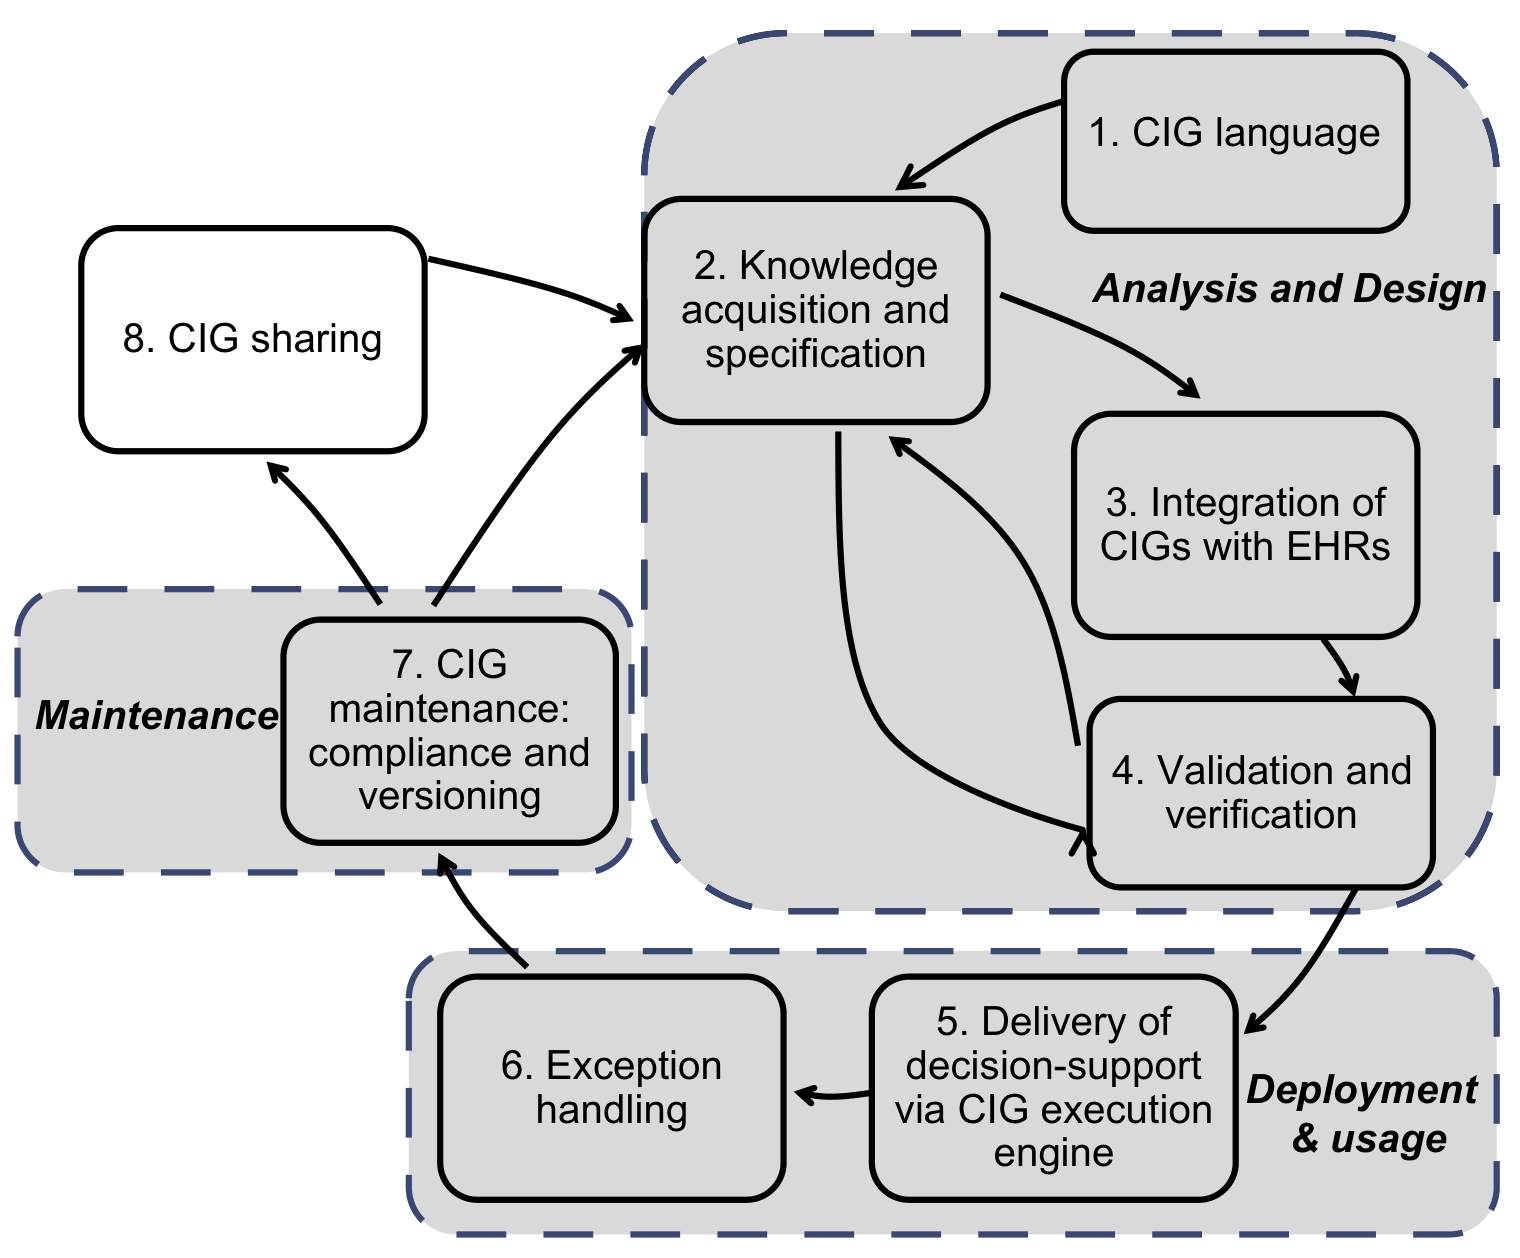
\includegraphics[width=\textwidth]{cpg-topics}
%  \caption{\CDSSs{} Research Themes}\label{fig:cpg-research-topics}
%\end{wrapfigure}
%
%\paragraph{Gap between specification and implementation:}
%
%To develop the \CIG{}, software developers rely on clinicians to interpret the
%non-executable \BPG{} and communicate
%the intended semantics to them. Thus, the non-executable \BPG{} serves as a functional specification for
%the \CIG{}, i.e. the implementation. In such safety-critical systems, it is
%imperative that the implementation, i.e. the \CIG{}, conforms to its
%specification, i.e., the \BPG{}. To address this, the \CIG{} is tested by
%putting the \CDSS{} through clinical simulations. But, while testing reduces
%the risk of non-conformance, it does not completely eliminate it.
%
%\paragraph{Formal semantics and analysis tools:}
%
%Given the safety-critical nature of \CDSSs{}, it is vital for \CIG{} languages
%to have complete formal semantics and formally-verified execution engines and
%analysis tools. This need has already been recognized in existing literature
%\cite{SuttonAMIA03, ShaharAMIA96}. It's also vital to ensure that
%associated tools are kept up to date as the language evolves.
%
%\paragraph{Holistic system safety:}
%
%While the safety critical nature of \CDSSs{} neccessitates
%\CIG{} languages to have comprehensive support for verification using
%tools like model checkers and deductive verifiers, certain challenges
%specific to \CDSSs{} require support beyond traditional techniques.
%
%Actions performed by a \CDSS{} can either be \emph{programming-oriented}
%or \emph{clinically-oriented} \cite{BoxwalaJBI04}. \emph{Programming-oriented}
%actions are peformed by executing the \CIG{} itself. For example,
%using patient parameters, or health records to make a reccomendation or diagnosis,
%or to raise a warning. \emph{Clinically-oriented} actions on the other hand
%are ones that involve a clinician. For example, in the case of \ACLS{},
%the \CDSS{} recommends that Cardiopulmonary Resuscitation (\CPR{}) be performed
%for a certain length of time. Such actions can only be performed by clinicians,
%and the \CDSS{} assumes that the recommended action was indeed performed before
%moving resuming guidance.
%
%For correctness, both categories of actions must be completed
%successfully. While traditional formal reasoning techniques can be employed
%to establish correctness of \emph{programming-oriented} actions, the same
%cannot be used to reason about \emph{clinically-oriented} ones.
%Thus, a mechanism that allows some guarantees about clinically-oriented is
%desirable.

\subsection{Proposed Approach}

This proposal aims to systematically address aforementioned challenges
using a \emph{semantics-first} approach. At the core of this approach
is a novel language for writing \BPGs{} in a \emph{computer interpretable}
manner called \MediK{}. By being \emph{comprehensible} to domain experts in medicine, \MediK{}-based
Computer Interpretable Guidelines (\CIGs{}) can serve as both the
non-executable \BPG{}, and the \BPGLogic{} of a \CDSS{}, eliminating any
\emph{specification-implementation gap}. Morover, any changes to the
\CIG{} are reflected immediately in the \CDSS{}.

\MediK{} merges the state-of-art in modeling and verifying concurrent systems and
\CIG{} languages to address the \emph{complexity} of \CDSSs{}.
A \MediK{} program consists of concurrently executing instances of
Finite State Machines (\FSMs{}) that interact by passing messages.
This enables a medical workflow, typically expressed using a flowchart-like
notation, to be naturally translated to \FSM{}. Event passing between machines
enables modeling inter-workflow interactions. \MediK{} treats
external agents as \FSMs{} - any external interaction occurs
through messages. This provides a \emph{uniform way} of incorporating
\emph{external agent}. For analysis, external agents are modeled as \emph{ghost}
\FSMs{} that support \emph{non-determinism}. \emph{Ghost} machines are discarded
at runtime, and any properties established using such machines are guaranteed
to hold as long as the external components conform to their \emph{ghost models}.

By \emph{semantics-first}, we mean that \MediK{}
has a \emph{complete, formal semantics}  from which tools such as an interpreter, model checker,
and deductive verifier are derived in a \emph{correct-by-construction}
manner. \MediK{} can rapidly evolve to incorporate feedback from
medical domain experts, as once the formal semantics are updated, the
tools evolve automatically.

\MediK{} has been used to implement a real-word \CDSS{} for screening and
management of pediatric sepsis, and establish said \CDSS{} satisfies desired
safety properties. To the best of our knowledge, it is the first system
for sepsis management with formal safety guarantees.

While \MediK{} presents a promising direction towards developing safe real-world
systems, realizing its full potential requires addressing the following research
challenges (RCs):

\paragraph{RC 1 (Design):} Is \MediK{}'s design conducive to expressing diverse \BPGs{}?

\BPGs{} can vary greatly by scope and purpose. For instance,
consider differences between the \BPGs{} for managing cardiac
arrest and sepsis. The \BPG{} for cardiac arrest can be
succinctly depicted by a single workflow. On the other hand, the \BPG{} for
screening and management of sepsis involves multiple workflows with complex
inter-workflow interactions.
This proposal seeks to answer whether \MediK{}'s
design can adequately accomodate diversity in \BPGs{}, without
compromising on readability. To this end, we plan to collaborate with
experts in medicine to ensure that the language meets their needs.
The \emph{semantics-first} approach is particularly
well-suited for designing the language, as updates to the language
only require changes to the semantics. As tools are derived from the semantics,
they update automatically.

\paragraph{RC 2 (Ecosystem):} Does \MediK{} have a mature
set of tools that enable building safe \CDSSs{}?

\MediK{} has a complete executable formal semantics, from which
its tools are derived in a \emph{correct-by-construction} fashion.
But, as real-world \BPGs{} are complex, establishing appropriate safety and liveness properties using
said tools presents various challenges. The proposal seeks to build on
\MediK{}'s toolchain to support verification of desired safety and liveness
properties of large \BPGs{}.

While $\K$ derived tools enable execution and analysis of \MediK{} programs,
certain \BPG{}-specific requirements may not have direct $\K{}$ equivalents.
In such cases, this proposal seeks to develop new semantics-based tools within
the $\K{}$ ecosystem, that are vital in \MediK's context, but may also have
applications for other $\K$-based languages.
For instance, visual representations of \MediK{} programs can
significantly improve comprehensibility of \MediK{} programs to medical domain
experts. This proposal seeks to expand on techniques
such as semantics-based compilation that can be used to extract information such
as basic blocks from code to generate \emph{correct-by-construction} visual
representation of programs in any language.

\paragraph{RC 3 (Applications):} Can our approach be used to build real-world
\CDSSs{}? How can \MediK{} improve \CDSSs{} effectiveness?

While \MediK{} has been used to implement a real-world,
this proposal seeks to establish that our approach can be used to build
other real-world \CDSSs{}. By real-world, we mean \CDSSs{} that are
capable of consideration for clinical trials at hospitals. Note that we
intend to use clinical-trial worthiness as an indicator of the effectiveness
of \MediK{}, not the result of the trial itself.
Clinical-trial worth systems need to be integrated into existing hospital care-flow.
This involves handle hospital-specific variations, such as
diversity in data sources and health records. This proposal seeks to
develop the \MediK{} ecosystem to a point where it can be used to build
such systems.

This proposal also seeks to develop new \CDSS{} capabilities enabled by the
\emph{semantics-first} approach. In particular, our approach
enables the following capabilities:

\begin{itemize}
  \item \textbf{Guideline Adherence Proofs:} Execution of a
\MediK{} \BPG{} is simply a proof in Matching Logic (ML), the logic
underlying the $\K{}$ framework, using the semantic rules as axioms.
Said proofs can be checked by an external ML proof-checker.
In \MediK{}'s case, execution proofs can serve as evidence of adherence to best practices during treatment.
Moreoever, zero-knowledge proofs can allow hospitals to establish
conformance to best practices, without divulging sensitive information
such as \emph{patient data} or \emph{specific treatment}
  \item \textbf{Safe Incorporation of Artificial Intelligence (AI):}
Advances in AI have applications in medicine. AI-based components
can enable early detection and targed treatment of medical conditions.
However, integrating such systems \emph{safely} remains a challenge,
\emph{hallucinations} in AI-based systems can lead to serious consequences.
We seek to explore \emph{safe} incorporation of AI-based systems into cafe-flow using
a simplex-based approach, where recommendations from an AI-based component are
\emph{checked} against known best practices before they're enacted.
If the recommendation is determined to be unsafe, a fallback action is enacted
instead.
\end{itemize}


